\chapter{Introduction}

%Channel limit
%
%URC
%Deep fade
%drop out
%5G

For all types of communication an important aspect is the channel through which the message is transmitted, for wireless communication, this is even more the case. The transmission of the message can be done in different environments, which have different impacts on the received signal. Common for all the environments is they introduce fading, which if not accounted for can have devastating effects for the transmission. 

Fading occurs when multipath propagation is present, that will introduce points in space where the waves adds either constructively or destructively, as can be seen on \autoref{intro_fading}. The constructive spots is not of much interest as it is only a couple of dB's difference, however the destructive interference can create spots with losses that borders minus infinite dB's. These spots are called deep fades and is is where the communication might suffer a drop out. A drop out occurs if the transmitted signal drops below the RX sensitivity level so the signal is lost. There are different tools to heighten the chance for the RX to receive signals that drops low and therefore increase the reliability of the communication link


\begin{figure}[H]
\centering
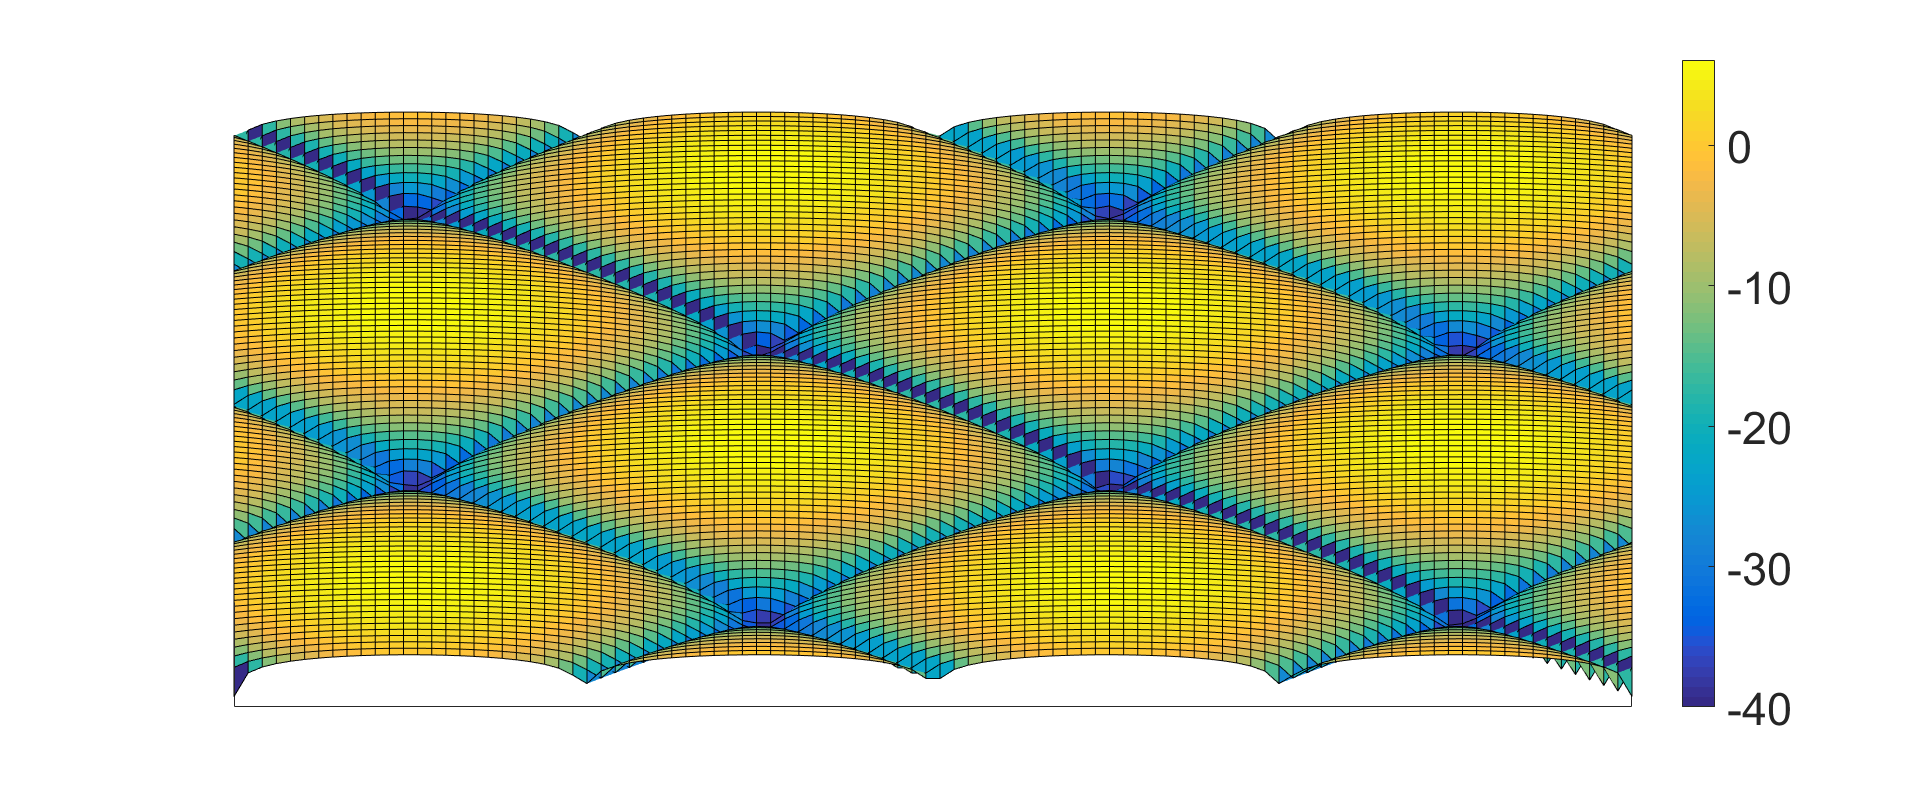
\includegraphics[width=\textwidth]{figures/intro_fading.png}
\caption{Fading gain from two wave fronts meeting, the deep fade spots have been elevated to allow for a better color resolution.}
\label{intro_fading}
\end{figure}

\section{Motivation}
With the development of the 5G wireless cellular network, a new concept have been introduced, \gls{URC}. Where earlier networks have run with a drop out probability of 0.1\%, with URC the drop out probability shall be under 0.001-0.0001\%. By having a better reliability, there a higher chance that some new application can be used on the cellular network. 
Some of these application could be communications between self driving cars, where short message about position and speed can be send to other cars in the area, with low chance of needing re-transmission, which is importing in case of high alert situations. Other system that can gain advantages with a higher reliability communication link, is system, where the communication window is very small and therefore there is not time to re-transmit or using a lot of error coding.


A problem about this is that to get this URC scenario, something have to be done to the channel. A way to get higher reliability is to transmit with a higher power level, so there gets a higher \gls{SNR} on the communication link. But even if the overall signal is higher, there will still be problem with fading in some points in space. 


\begin{figure}[H]
\centering
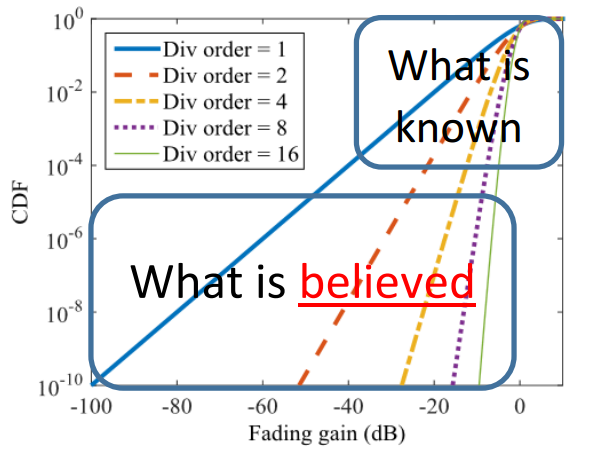
\includegraphics[width=0.65\textwidth]{figures/fading_gain.png}
\caption{\gls{CDF} of fading gain in different channel environments.}
\label{fading_gain}
\end{figure}


\section{Project outline}





